\section{Features}

Uno dei componenti essenziali del metodo di Viola e Jones è l'utilizzo di un sistema di feature molto semplice ed un modo altrettanto veloce per calcolarle.

Viene inizialmente definita una \emph{detection window} di dimensione prefissata (generalmente 24 x 24) e si fa scorrere quest'ultima lungo tutta l'immagine da analizzare alla ricerca di facce. In ciascuna posizione vengono analizzate un'insieme di feature locali, in questo caso le Haar-like.

\subsection{Le features Haar-like}

Le features Haar-like consistono in 2 o più rettangoli bianchi o neri adiacenti all'interno della \emph{detection window}. A partire da una configurazione di rettangoli viene calcolata la differenza delle somme dei pixel sottostanti una regione bianca e quelli sottostanti ad una regione nera. In questo modo è possibile identificare zone in cui vi è un contrasto nella direzione indicata dalla posizione dei rettangoli. Una zona omogenea infatti darà valori circa prossimi a 0.

Sia $X$ un'immagine. Chiamiamo $W$ l'insieme dei pixel sottostanti una regione \textit{bianca} e $B$ l'insieme dei pixel sottostanti una regione \textit{nera}. Il valore della feature è ottenuto tramite

$$
f = \sum_{i \in W} x_i - \sum_{j \in B} x_j
$$

Le features utilizzate nel metodo di Viola e Jones sono di 5 tipi diversi, come mostrato in Figura \ref{fig:haar}.

\begin{figure}[h]
\begin{center}
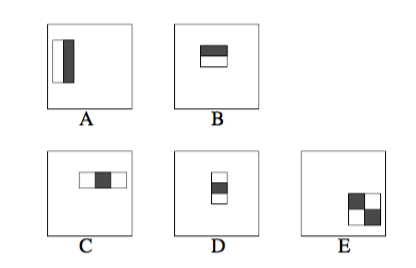
\includegraphics[width=0.35\textwidth]{images/haar}
\end{center}
  \caption{I 5 tipi diversi di Haar-like features utilizzati}
\label{fig:haar}
\end{figure}

Il numero totale di features di tutti e 5 i tipi scalati e traslati all'interno di una \emph{detection window} 24 x 24 è di 162,336. Come nell'implementazione di OpenCV sono state però considerate solo le features con un area superiore a 32 pixels: questo per evitare di andare a considerare delle regioni troppo piccole e irrilevanti ai fini del riconoscimento. Con queste particolari restrizioni il numero totale di features si riduce a 108,490. 

\subsection{Immagini integrali}

Al fine di poter riconoscere i volti in tempo reale è necessario poter valutare queste features in poco tempo. Per fare questo Viola e Jones hanno introdotto una nuova rappresentazione dell'immagine chiamata \emph{immagine integrale}.

L'immagine integrale è costruita utilizzando una matrice della stessa dimensione dell'immagine originale con associata a ciascun elemento la somma dei valori dei pixel che si trovano sopra e a sinistra del pixel corrispondente.

Sia $i$ l'immagine originale e $I$ la sua rappresentazione integrale. Un generico elemento della matrice integrale si trova con:

$$
I(x, y) = \sum_{x' \leq x, y' \leq y} i(x', y')
$$

E' possibile giungere alla costruzione di questa matrice iterativamente utilizzando le seguenti due formule:
$$
s(x, y) = s(x, y - 1) + i(x, y)
$$
$$
I(x, y) = I(x - 1, y) + s(x, y)
$$

\begin{figure}[h]
\begin{center}
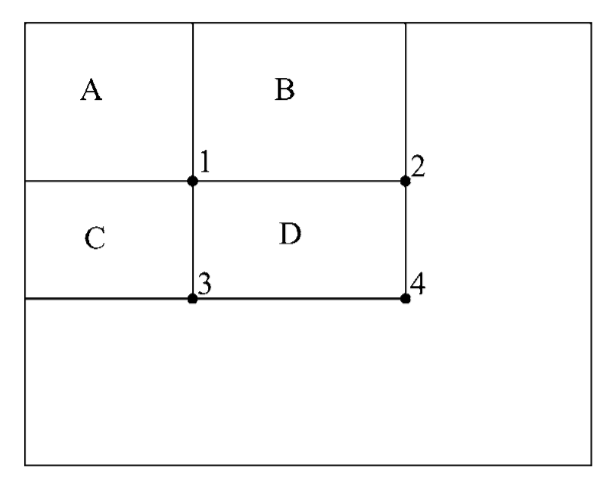
\includegraphics[width=0.35\textwidth]{images/integral}
\end{center}
  \caption{Calcolo della somma dei pixel in una regione rettangolare}
\label{fig:integral}
\end{figure}
A questo punto, data la regione rettangolare $D$, per calcolare la somma dei pixel all'interno della stessa sarà sufficiente valutare
$$
S = I(x_4, y_4) + I(x_1, y_1) - I(x_2, y_2) - I(x_3, y_3)
$$
dunque è un calcolo estremamente veloce.


